\subsection{WebApp - BackEnd}\label{sec:WebAppBackEnd}
WebApp - BackEnd is a Middleware that runs on the server. This Middleware (server-side software) facilitates client-server connectivity, forming a middle layer between the app(s) and the network: the server, the database, the operating system, and more. It receives requests from the clients (in this case, the WebApp - FrontEnd), and contains the logic to send the appropriate data back to the applicant, over HTTP and REST.  These are the main conventions that provide structure to the request-response cycle between clients and servers. The pair of an HTTP verb and a URI is called a route and matching them based on a request is called routing.

WebApp - BackEnd is an application build with Node.js, an application platform where developers can write Javascript programs that are compiled, optimized and interpreted by the V8 virtual machine. Node.js can create quick, reliable websites and products in much efficient manner. Node.js backend is great for organisations seeking to rapidly prototype an idea. Developing easy to scale real time applications in other technologies is bit difficult, but JavaScript technologies made it easier.

The WebApp - BackEnd is composed by the API Gateway, Service Layer and Resource Locator more detailed below.

\subsubsection{API Gateway}\label{sec:APIGateway}
API Gateway is a managed service that enables easily create, publish, maintain, monitor and secure REST APIs to act as a "gateway" for applications to access data, business logic, or functionality in the backend services, such as workloads. The API Gateway provides a simple uniform view of external resources to the internals of an application. It manages all tasks involved in receiving and processing API calls, including traffic management, authorization and access control, monitoring and management of API versions.

\begin{figure}[htbp]
\begin{center}
  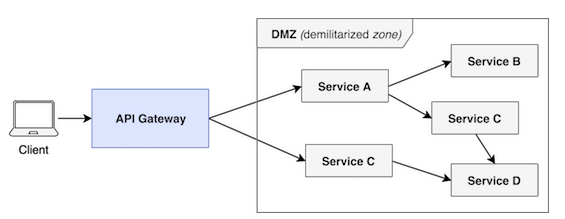
\includegraphics[scale=0.75]{images/apigateway.png}
\caption{API Gateway.}
\label{default-regular2}
\end{center}
\end{figure}

An API is a collection of clearly defined methods of communication between different software components. More specifically, a Web API is the interface created by the back-end: the collection of endpoints and the resources these endpoints expose. A Web API is defined by the types of requests that it can handle, which is determined by the routes that it defines, and the types of responses that the clients can expect to receive after hitting those routes. One Web API can be used to provide data for different front-ends. Since a Web API can provide data without really specifying how the data is viewed, multiple different HTML pages or mobile applications can be created to view the data from the Web API.

Basically, the Gateway is an interface that receives calls to its internal systems, being a large gateway. 

It can act in five different ways:

\begin{itemize}
\item Filter for call traffic from different media (web, mobile, cloud, among others);
\item Single gateway to the various APIs you want to expose;
\item Essential component of API management, as API Suite;
\item Router: API and Rate Limit traffic router;
\item Security engine with authentication, logging and more.
\end{itemize}

Gateway access can be done from many different devices. Therefore, it must have the power to unify outgoing calls and be able to deliver to the user content that can be accessed from any browser and system. The 6 Benefits of a Gateway API:

\begin{enumerate}
\item Application Layer Separation and different requests:
One of the best benefits of this layer is that a gateway can clearly separate implemented APIs and microservices from the people who will actually use them.
\item Increased simplicity for the consumer: Using a Gateway, is possible to show to end user a unique front end with an API collection, and can be much more transparent with API users.
\item Development Improvement: Separation of purposes and functionality not only makes development focus much more on what is really needed, but also helps the server withstand the information demand for the services used. For example, a service that is called a few times a day needs fewer resources than a service called all the time, making the most of the machine's performance.

\item Buffer Zone against attacks: By utilizing multiple standalone Gateway-controlled services, any attack on the application will not affect the overall system, just that service, keeping everything running smoothly. This is the Buffer Zone. In addition to security, this strategy makes it much simpler for the user, as all other features remain normal, not causing stress.

\item Dedication of Services in Favor of User Experience: With the API service independence strategy, a developer can have all the documentation needed to use in a much simpler way, optimizing their time and dedicating themselves exclusively to their activity. This way is possible to usage SDKs for each API separately to make documentation as specific as possible.

\item Activity log anticipating errors: Since all calls to services will go through the Gateway, controlling them all is very simple. This type of log can give the owner of the API a very high power. With it, is possible to find all the errors that can bring down any service, and even who is responsible for a good consumption of the API. This way is easier to predict the number of possible calls avoiding any problems for users.

\end{enumerate}

Gateways as a Security Feature: In the APIs world, one of the most subject talked about issues is always security, and having an API Gateway is one of the best solutions on the market to get full control of API’s, because this pattern addresses the so-called CIA (Confidentiality, Integrity, Availability) almost flawlessly.

\subsubsection{Service Layer}\label{sec:ServiceLayer}
A Service Layer defines an application's boundary [Cockburn PloP] and its set of available operations from the perspective of interfacing client layers. It encapsulates the application's business logic, controlling transactions and coordinating responses in the implementation of its operations.

Enterprise applications typically require different kinds of interfaces to the data they store and the logic they implement: data loaders, user interfaces, integration gateways, and others. Despite their different purposes, these interfaces often need common interactions with the application to access and manipulate its data and invoke its business logic. The interactions may be complex, involving transactions across multiple resources and the coordination of several responses to an action. Encoding the logic of the interactions separately in each interface causes a lot of duplication.

Using service layer pattern provides some benefits:

\begin{enumerate}
\item Centralizes external access to data and functions.
\item Hides (abstracts) internal implementation and changes.
\item Allows for versioning of the services.
\end{enumerate}

The service layer acts as an orchestrator, controlling the flow of incoming and outcoming information requests and responses. Orchestration allows to directly link process logic to service interaction within workflow logic. This combines business process modeling with service-oriented modeling and design, realizing workflow management through a process service model. Orchestration brings the business process into the service layer, positioning it as a master composition controller.

\subsubsection{Resource Locator}\label{sec:ResourceLocator}

Resource locators are components that abstracts the persistence layer. Their job is to provide an object that can help services to discover and persist information from/to the Data Storage Module. Information can be stored in the Blockchain, Filesystem or Database and resource locators should know exactly where get/put data within them.  